\section{Funktionen}\label{sec:funktionen}
\setcounter{page}{1}

Für die Beschreibung von Vorgänge, Situationen oder charakteristische Eigenschaften werden zur Darstellung/Modellierung häufig Funktionen benutzt.

\subsection{Einführung}\label{subsec:einfuhrung-funktionen}

\begin{definition}{Funktionen}
    Eine Funktion $f$ ist eine Vorschrift, die jedem Element aus einer Menge $D$ genau ein Element einer Menge $W$ zuordnet.
    Die Menge $D$ wird als \emph{Definitionsbereich} bezeichnet, die Menge $W$ wird als \emph{Wertebereich} bezeichnet.
\end{definition}

\subsection{Darstellungen von Funktionen}\label{subsec:darstellungen-von-funktionen}

Es gibt verschiedene Möglichkeiten, Funktionen darzustellen.
\begin{itemize}
    \item Durch eine Tabelle: $\quad$
    \begin{tabular}{|c|c|c|c|c|c|c|c|c|c|c|}
        \hline
        $x$    & 1 & 2 & 3 & 4  & 5  & 6  & 7  & 8  & 9  & 10 \\
        \hline
        $f(x)$ & 4 & 6 & 8 & 10 & 12 & 14 & 16 & 18 & 20 & 22 \\
        \hline
    \end{tabular}
    \item Durch eine Formel: $y = f(x) = 2x + 2$
    \item Durch einen Graphen:
    \begin{center}
        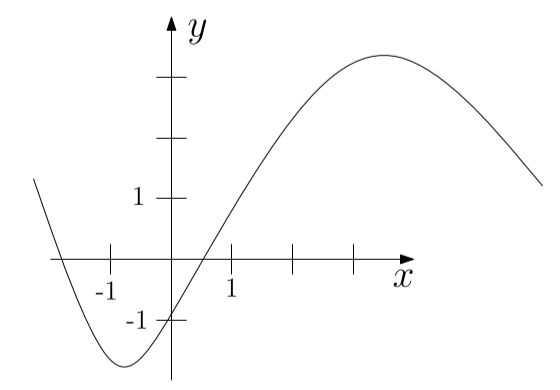
\includegraphics[scale=0.5]{function-graph}
    \end{center}
\end{itemize}

\subsubsection{Nullstellen einer Funktion}

Eine Stelle $x \in D$ mit $f(x) = 0$ heisst \emph{Nullstelle} der Funktion $f$.
Anschaulich ist eine Nullstelle ein Schnittpunkt des Graphen mit der $x$-Achse.
Nullstellen spielen bei vielen Algorithmen, welche zur numerischen Lösung von Gleichungen verwendet werden, eine wichtige Rolle.

\subsection{Operationen mit Funktionen}\label{subsec:operationen-mit-funktionen}

Da die Wertebereiche zweier Funktionen jeweils in $\R$ liegen, lassen sich Funktionen addieren, multiplizieren, etc.
Wir benutzen dieselben Symbole wie bei der Addition, Multiplikation, etc.\ von Zahlen;
streng genommen haben sie hier aber eine andere Bedeutung: Sie beziehen sich auf die Ausführung einer Operation für unendlich viele Werte.

\begin{definition}{}
    Wir betrachten eine beliebige Menge $D$ und zwei Funktionen $f : D \rightarrow \R$ mit $x \mapsto f(x)$ und $g : D \rightarrow \R$ mit $x \mapsto g(x)$.
    Dann können wir die folgenden Operationen definieren:
    \begin{itemize}
        \item Addition: $f + g : D \rightarrow \R$ mit $x \mapsto f(x) + g(x)$
        \item Subtraktion: $f - g : D \rightarrow \R$ mit $x \mapsto f(x) - g(x)$
        \item Multiplikation: $f \cdot g : D \rightarrow \R$ mit $x \mapsto f(x) \cdot g(x)$
        \item Division: $\frac{f}{g} : D \rightarrow \R$ mit $x \mapsto \frac{f(x)} {g(x)} \quad\quad$ falls $g(x) \neq 0$ für alle $x \in D$
        \item Skalierung: $c \cdot f : D \rightarrow \R$ mit $x \mapsto c \cdot f(x) \quad\quad$ für ein fixes $c \in \R$
    \end{itemize}
\end{definition}

\subsection{Komposition}\label{subsec:komposition}

\begin{definition}{Komposition}
    Für zwei gegebene Funktionen $f : A \rightarrow B$ und $g : B \rightarrow C$ ist die Funktion $g \circ f : A \rightarrow C$ definiert durch \[(g \circ f)(x) = g(f(x))\]
    Diese neue Funktion heisst \emph{Komposition} von $f$ und $g$.
\end{definition}

\textbf{Bemerkung:} Zuerst wird die Funktion angewendet, die \emph{rechts} steht!
Ausserdem $f \circ g \neq g \circ f$.

\textbf{Beispiel:} Bestimme die Komposition mit $f(x) = 3x + 7$ und $g(x) = \sqrt{x}$: $(g \circ f)(x) = g(f(x)) = \sqrt{3x + 7}$.

\subsection{Umkehrfunktion}\label{subsec:umkehrfunktion}

\begin{definition}{Umkehrfunktion}
    Eine Funktion $f$ heisst \emph{injektiv}, wenn aus $x_1 \neq x_2$ stets $f(x_1) \neq f(x_2)$ folgt.
    In diesem Fall gibt es für $f$ eine \emph{Umkehrfunktion} $g$ mit \[g(y) \coloneqq x\], wobei $x$ die Eigenschaft $f(x) = y$ hat.
    Sie wird auch mit $f^{-1}$ bezeichnet.
\end{definition}

\textbf{Beispiel:} Bestimme die Umkehrfunktion von $f(x) = \frac{3}{2x-5}$: \[y = \frac{3}{2x-5} \Rightarrow y(2x-5) = 3 \Rightarrow 2xy = 3 + 5y \Rightarrow x = \frac{3 + 5y}{2y} \Rightarrow g(x) = \frac{3+5y}{2y}\]

\subsection{Summenzeichen}\label{subsec:summenzeichen}

Im Zusammenhang mit Funktionen kommt ab und zu das Summenzeichen $\sum$ vor.
Sie ist definiert als \[\sum_{i=1}^n a_i = a_1 + a_2 + \dots + a_n\]

\begin{definition}{Rechenregeln für das Summenzeichen}
    \begin{alignat*}{3}
        &(1) \sum_{k=s}^{n} (c \cdot a_k) &&= c \cdot a_s + c \cdot a_{s+1} + \dots + c \cdot a_n &&= c \cdot \sum_{k=s}^{n} a_K \\
        &(2) \sum_{k=s}^{n} (a_k + b_k) &&= a_s + b_s + a_{s+1} + b_{s+1} + \dots + a_n + b_n &&= \sum_{k=s}^{n} a_k + \sum_{k=s}^{n} b_k \\
        &(3) \sum_{k=s}^{n} a_k + \sum_{k = n + 1}^{m} a_k &&= \sum_{k = s}^{m} a_k = \sum_{r = s}^{m} a_r = \sum_{i = s}^{m} a_i \\
    \end{alignat*}
\end{definition}

\textbf{Bemerkung:} \[\sum_{k=0}^n (a_k \cdot b_k) \neq \left( \sum_{k=0}^n a_k \right) \cdot \left( \sum_{k=0}^n b_k \right)\]

\vspace{-\topsep}

\subsubsection{Spezielle Summenformeln}

\begin{multicols}{2}
    \begin{definition}{Arithmetische Summenformel}
        \[\sum_{k=1}^n k = \frac{n(n+1)}{2}\]
    \end{definition}
    \begin{definition}{Summe der Quadratzahlen}
        \[\sum_{k=1}^n k^2 = \frac{n(n+1)(2n+1)}{6}\]
    \end{definition}
\end{multicols}